\documentclass[border=3pt]{standalone}
% Preâmbulo compartilhado pelos diagramas TikZ da aula 5 de IHC (Processos de Design)
\usepackage[T1]{fontenc}
\usepackage[utf8]{inputenc}
\usepackage{lmodern}
\usepackage{amsmath}
\usepackage{xcolor}
\usepackage{tikz}
\usetikzlibrary{arrows.meta,angles,quotes,decorations.pathmorphing,calc,
                positioning,shapes.geometric,shapes.misc,backgrounds,fit,
                math}

% Paleta (mesma dos SVGs originais)
% Paleta da disciplina de IHC: acento roxo (#755099), da capa do livro.
% (o nome "dblue" é mantido para não alterar todos os diagramas)
\definecolor{dblue}{HTML}{755099}
\definecolor{dorange}{HTML}{B3541E}
\definecolor{dgreen}{HTML}{4A7C59}
\definecolor{dred}{HTML}{9C4B4B}
\definecolor{dcream}{HTML}{F4F1EA}
\definecolor{dshade}{HTML}{DDD7C9}

% Função gaussiana (não normalizada por padrão de escala visual)
\pgfmathdeclarefunction{gauss}{3}{%
  \pgfmathparse{1/(#3*sqrt(2*pi))*exp(-((#1-#2)^2)/(2*#3^2))}%
}

% Estilos comuns (prefixo d... para não colidir com chaves internas do pgf)
\tikzset{
  >={Stealth[length=2mm]},
  dguide/.style={gray!55, dashed, line width=0.4pt},
  daxis/.style={gray!60, line width=0.7pt, ->},
  dbody/.style={fill=black!3, draw=black!80, line width=1pt},
  dacc/.style={draw=dblue, line width=1pt},
  dlbl/.style={black!55, font=\small},
  dsub/.style={black!45, font=\footnotesize},
  dstate/.style={circle, draw=black!80, fill=dcream, line width=1pt,
                 minimum size=17mm, font=\large, inner sep=1pt},
  dobs/.style={circle, draw=black!80, fill=dshade, line width=1pt,
               minimum size=14mm, font=\large, inner sep=1pt},
  dbox/.style={rounded corners=2pt, draw=black!80, fill=dcream, line width=1pt,
               align=center, inner sep=6pt},
  dop/.style={circle, draw=black!80, fill=white, line width=1pt,
              minimum size=6mm, inner sep=0pt, font=\small},
  dtrans/.style={->, dblue, line width=1pt},
  dmeas/.style={->, dorange, line width=1pt},
  dcurve/.style={line width=1pt, dblue},
  dcurveb/.style={line width=1.4pt, dorange},
}

\begin{document}
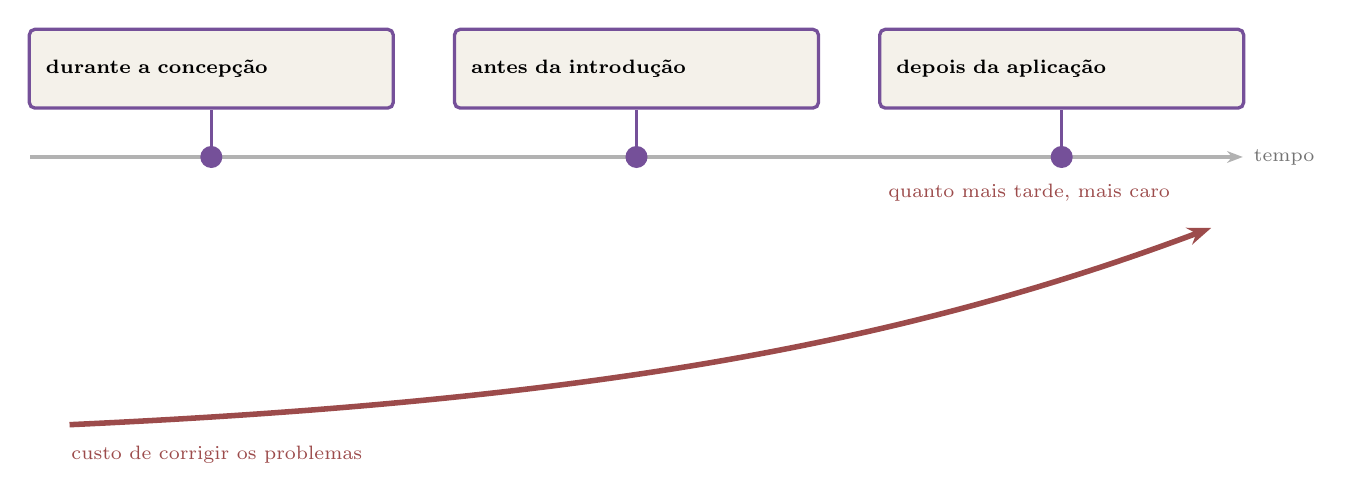
\begin{tikzpicture}[x=1cm,y=1cm,
   mom/.style={dbox, text width=4.2cm, minimum height=1.0cm, font=\scriptsize, align=left}]

  \draw[daxis, line width=1.4pt] (0,0) -- (15.4,0) node[right, dlbl, font=\scriptsize] {tempo};

  \node[mom, draw=dblue, line width=1.2pt, anchor=south] at (2.3,0.6) {\textbf{durante a concepção}};
  \node[mom, draw=dblue, line width=1.2pt, anchor=south] at (7.7,0.6) {\textbf{antes da introdução}};
  \node[mom, draw=dblue, line width=1.2pt, anchor=south] at (13.1,0.6) {\textbf{depois da aplicação}};
  \foreach \x in {2.3,7.7,13.1} { \fill[dblue] (\x,0) circle (0.14); \draw[dblue, line width=1pt] (\x,0) -- (\x,0.6); }

  % custo de correção (sobe com o tempo)
  \draw[dred, line width=2pt, -{Stealth[length=3mm]}] (0.5,-3.4) .. controls (7,-3.1) and (11,-2.4) .. (15.0,-0.9);
  \node[dred, font=\scriptsize, anchor=north west] at (0.4,-3.55) {custo de corrigir os problemas};
  \node[dred, font=\scriptsize, anchor=east] at (14.6,-0.45) {quanto mais tarde, mais caro};

\end{tikzpicture}
\end{document}
